% =====================================================================
% TECHNICAL SUMMARY -- for advisor review. NOT a submission draft.
%
% Longer documents this is condensed from:
%   paper/master/haatim_hsgs_master.tex   (13 pp., complete research record)
%   paper/master/MASTER_PAPER_AUDIT.md    (every number vs. its store)
%   paper/merged/haatim_hsgs_bounds_and_effective_rank.tex (5 pp., SPL draft)
%
% DATA HYGIENE (load-bearing). Three experiment families appear here and are
% NEVER pooled. Every numeric claim carries a % SRC comment naming its store.
%   [B3]  results/track_b/b3/          N in {8,16,32} x P in {10,30} x 6 SNR
%                                      400 trials/pt, RSR 12 dB, T=50, n_cz=4
%   [EXT] trackB_hankel_emgs/results/  P=30 only, 7 SNR pts, 600/400/200 trials
%   [TD]  results/track_d/partB9/      N in {16,32,64}, P=20, adaptive order,
%                                      n_cz=1, T=100, SNR ~ U[-10,20]
% One Cadzow sweep and four Cadzow sweeps define DIFFERENT operators, so TD
% and B3 numbers are never compared as measurements of the same estimator.
% =====================================================================
\documentclass[conference]{IEEEtran}
\IEEEoverridecommandlockouts

\usepackage{amsmath,amssymb,amsfonts}
\usepackage{graphicx}
\usepackage{booktabs}
\usepackage{url}
\usepackage[hidelinks]{hyperref}

\DeclareMathOperator{\rank}{rank}
\newcommand{\rmax}{r_{\max}}
\newcommand{\reff}{r_{\mathrm{eff}}}
\newcommand{\bG}{\mathbf{G}}
\newcommand{\bS}{\mathbf{S}}
\newcommand{\bB}{\mathbf{B}}
\newcommand{\bW}{\mathbf{W}}
\newcommand{\bZ}{\mathbf{Z}}
\newcommand{\bg}{\mathbf{g}}
\newcommand{\Hank}{\mathcal{H}}
\newcommand{\dHS}{\Delta_{\mathrm{HS}}}

\begin{document}

\title{Hankel-Structured Channel Estimation for\\
Rydberg Atomic Receivers:\\
\large Effective-Rank Scaling of the Structural Gain}

\author{\IEEEauthorblockN{Abdullah Haatim}
\IEEEauthorblockA{Department of Electrical and Electronics Engineering\\
Birla Institute of Technology and Science, Pilani --- Pilani Campus, India\\
f20220519@pilani.bits-pilani.ac.in}}

\maketitle

\begin{abstract}
A Rydberg atomic receiver reads a radio field through an optical transition
whose response follows field magnitude, so multi-user channel estimation
becomes a phase-retrieval problem in which the noise sits inside the modulus.
The established baseline, Gerchberg--Saxton with an EM refinement (EM-GS),
treats the channel as unstructured across array elements. We investigate adding
a physics-based structural prior: for a uniform linear array the Hankel lifting
of each channel column is low rank, so we insert a low-rank Hankel projection
into the EM-GS iteration, with the projection order selected from held-out
pilots and disabled when the selected order reaches the array's Hankel rank
capacity. In simulation the resulting HS-GS estimator improves on EM-GS by
$2.27$--$3.04$~dB at $N=32$, $P=30$, but the gain is not universal: it is
negative at $N=8$ and decays to zero as the channel's normalised effective rank
approaches unity. Our results indicate that this normalised effective rank,
rather than array size or raw path count, is the coordinate that governs when
the prior helps; two frozen cross-generator predictions were met to $0.13$ and
$0.315$~dB. All results are simulation-only.
\end{abstract}

\begin{IEEEkeywords}
Rydberg atomic receiver, phase retrieval, channel estimation, Hankel matrix,
structured low-rank approximation, effective rank.
\end{IEEEkeywords}

% =====================================================================
\section{Problem}
% =====================================================================

A Rydberg atomic receiver detects a radio field through an optical transition
whose readout is proportional to field \emph{magnitude}
\cite{gong2025mag}. With an $N$-element array serving $K$
single-antenna users over $P$ pilot symbols, the receiver observes
\begin{equation}\label{eq:obs}
\bZ = \bigl|\,\bG\bS + \bB + \bW\,\bigr| \in \mathbb{R}_{\ge0}^{N\times P},
\end{equation}
where $\bG\in\mathbb{C}^{N\times K}$ is the unknown channel, $\bS$ the pilot
matrix, $\bB$ a known additive reference field (a local oscillator, needed to
break the sign ambiguity of a pure magnitude measurement), and $\bW$ circularly
symmetric noise. The modulus is applied \emph{after} the noise is added, so the
phase of the composite field is lost and \eqref{eq:obs} cannot be linearised
without changing the problem. Channel estimation is therefore biased phase
retrieval. The standard treatment alternates a magnitude substitution with a
least-squares update --- Gerchberg--Saxton \cite{gerchberg1972} --- and replaces
the hard substitution by the Rician conditional mean, giving EM-GS
\cite{cui2025,xu2025}, the baseline throughout this work.

\textbf{The gap we address.} EM-GS estimates $\bG$ as $2NK$ free real
parameters: nothing in the iteration relates one array element to the next.
But a uniform linear array (ULA) illuminated by a finite number of propagation
paths produces a channel with strong deterministic cross-element structure. We
investigate whether imposing that structure inside the phase-retrieval
iteration improves the estimate, and --- the question that occupies most of
this summary --- \emph{when} it does.

\textbf{Scope of the contribution.} None of the ingredients are new: Hankel
low-rank models, Cadzow's projection \cite{cadzow1988}, structured low-rank
approximation \cite{markovsky2008}, effective rank \cite{royvetterli2007}, and
rank-constrained estimation for atomic receivers \cite{xu2025} all predate this
work. To the best of our knowledge the \emph{combination} has not been
reported: a Hankel regulariser inside magnitude-only Rydberg EM-GS; order
selection that uses no oracle and abstains when the prior cannot be supported;
a characterisation of when the prior helps in terms of normalised effective
rank; and a prospective test of that characterisation on channel generators not
used to build it.

% =====================================================================
\section{Hankel Structure and the HS-GS Estimator}
% =====================================================================

\subsection{Why the structure exists}

For a ULA with $L_k$ propagation paths, the channel of user $k$ at element $n$
is a sum of complex exponentials in the element index,
\begin{equation}\label{eq:chan}
g_k[n] = \sum_{\ell=1}^{L_k}\alpha_{\ell,k}\,
e^{-j(n-1)\psi_{\ell,k}},\qquad \psi_{\ell,k}=\pi\sin\theta_{\ell,k}.
\end{equation}
Let $\Hank(\bg)$ be the $(N-p)\times(p+1)$ Hankel lifting of the column $\bg$.
Substituting \eqref{eq:chan} separates the exponential in the two indices, so
each path contributes exactly one rank-one outer product:
\begin{equation}\label{eq:rank}
\Hank(\bg_k)=\sum_{\ell=1}^{L_k}\alpha_{\ell,k}\,
\mathbf{v}_\ell\mathbf{w}_\ell^{\!\top}
\;\Longrightarrow\;
\rank\Hank(\bg_k)\le L_k .
\end{equation}
A finite-path ULA channel is thus \emph{exactly} low rank after lifting, while
noise and phase-retrieval error are not: they fill the Hankel spectrum.
Projecting an EM-GS estimate back toward a low-rank Hankel matrix should
therefore remove error the physics forbids while retaining signal it permits.
Two consequences shape everything that follows.

\textbf{The prior has a finite capacity.} Since $\Hank(\bg)$ is
$(N-p)\times(p+1)$, its rank cannot exceed
\begin{equation}\label{eq:cap}
\rmax(N)=\max_p \min(N-p,\;p+1)=\lceil N/2\rceil .
\end{equation}
If $L_k\ge\rmax(N)$ the constraint in \eqref{eq:rank} is vacuous. The value of
the prior is therefore bounded by aperture, and this is what makes the method's
benefit conditional rather than universal.

\textbf{The projection is approximate.} The intersection of the fixed-rank
matrices and the Hankel matrices is a non-convex variety; Cadzow's alternating
scheme \cite{cadzow1988} approaches it but the composite map is not an
idempotent projection onto it. Fig.~\ref{fig:spectrum} shows the residual
directly, and it upper-bounds how much structure the method can impose.

\begin{figure}[!t]
\centering
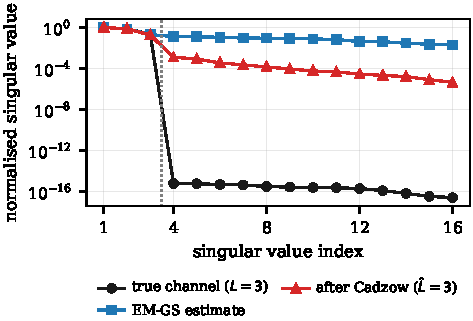
\includegraphics[width=0.86\columnwidth]{fig/fig4_hankel_spectrum.pdf}
% SRC: trackB_hankel_emgs/results/diagnostic_spectrum.json (family EXT),
% trial 0, seed 20250820, order forced to true L, n_cz=4.
% true_channel[3]=5.73e-16; em_gs_estimate[3]=0.130; after_cadzow[3]=1.24e-3.
\caption{\textbf{Why the prior exists, and what the projection achieves.}
[Family EXT, one illustrative realisation.] Normalised Hankel singular values
for one channel column, $N=32$, $L=3$, SNR $=5$~dB. The true channel is exactly
rank $L$ ($\sigma_4/\sigma_1=5.7\times10^{-16}$, the numerical-precision
floor). The EM-GS estimate has no such cliff ($\sigma_4/\sigma_1=0.130$) ---
noise fills the spectrum, so the estimate is not a sum of $L$ exponentials.
Four Cadzow sweeps restore a cliff at the correct index but only to
$1.2\times10^{-3}$: the structure is imposed \emph{approximately}, which caps
the attainable gain. Single realisation, shown for mechanism, not as a
statistical claim.}
\label{fig:spectrum}
\end{figure}

\subsection{HS-GS}

The proposed estimator inserts the projection into the exact EM-GS iteration:
\begin{center}
EM-GS update $\rightarrow$ Hankel lifting $\rightarrow$ rank-$\hat L$ Cadzow
projection $\rightarrow$ back to the channel domain $\rightarrow$ next EM-GS
update.
\end{center}
Everything else --- initialisation, iteration count, the Rician conditional
mean --- is unchanged. With the projection disabled, HS-GS reproduces EM-GS
bit for bit ($\max|\text{diff}|=0$, verified in the accompanying test suite), so
the projection is provably the only difference between them.

\textbf{Order selection without an oracle.} $\hat L$ is never taken from ground
truth. A fraction $\nu=0.3$ of the pilots is held out, each candidate order is
scored by the held-out residual, and the best is used for the full run. The
\emph{in-sample} residual cannot serve this purpose: constraining $\bG$ can only
worsen the fit to the pilots used for fitting, so an in-sample criterion always
prefers the largest candidate. One scalar $\hat L$ is shared by all $K$ users.

\textbf{Abstention.} If the selector returns $\hat L\ge\rmax(N)$, the
projection is the identity and is switched off. This is a designed behaviour,
not a failure mode: the estimator declines to impose structure the aperture
cannot support, and falls back exactly to EM-GS.

% =====================================================================
\section{Results}\label{sec:results}
% =====================================================================

Table~\ref{tab:fam} lists the three experiment families used below. They have
different array sizes, pilot counts, SNR grids, sweep counts and pooling rules,
and are \textbf{never} combined: each number below is tagged with the family it
comes from.

\begin{table}[!t]
\caption{The three experiment families. Different configurations; numbers from
one are not comparable to numbers from another as measurements of the same
estimator.}
\label{tab:fam}
\centering
\scriptsize
\setlength{\tabcolsep}{3pt}
\begin{tabular}{lll}
\toprule
Tag & Store & Configuration \\
\midrule
B3 & \texttt{results/track\_b/b3/} &
$N\!\in\!\{8,16,32\}$, $P\!\in\!\{10,30\}$, \\
 & & 6 SNR pts, 400 trials/pt, $n_{\mathrm{cz}}\!=\!4$ \\[2pt]
EXT & \texttt{trackB\_hankel\_emgs/} &
$P\!=\!30$ only, 7 SNR pts, \\
 & & $600/400/200$ trials, $n_{\mathrm{cz}}\!=\!4$ \\[2pt]
TD & \texttt{results/track\_d/partB9/} &
$N\!\in\!\{16,32,64\}$, $P\!=\!20$, adaptive \\
 & & order, $n_{\mathrm{cz}}\!=\!1$, SNR $\sim\mathcal{U}[-10,20]$ \\
\bottomrule
\end{tabular}
\end{table}

\subsection{Does HS-GS improve on EM-GS?}

At the principal operating point --- $N=32$, $K=3$, $P=30$, $400$ paired trials
per SNR point --- HS-GS improves on EM-GS by
% SRC: results/track_b/b3/N32_P30_snr*.npz, ratio-of-sums per point.
$+2.27$ to $+3.04$~dB across the tested sweep [B3]
(Fig.~\ref{fig:main}, left).

That gain deserves a comment, because EM-GS is not a weak baseline: against a
% SRC: results/track_b/constrained_crlb.json, N32_P30.
rank-one Rician bound computed on the same trials, EM-GS tracks the
\emph{unconstrained} CRLB to within $0.051$~dB for SNR $\ge5$~dB [B3]. Nearly
$3$~dB over an estimator that close to its bound looks contradictory until one
notes that the unconstrained bound treats $\bG$ as $2NK$ free parameters.
Restricting to the geometric manifold of \eqref{eq:chan} and applying the
constrained CRLB \cite{gorman1990,stoica1998} gives a bound $7.05$--$7.11$~dB
\emph{below} the unconstrained one here [B3]; that gap is the headroom the
prior reaches into, and HS-GS recovers part of it. Neither bound formally
governs the estimators plotted against it, since all are biased --- they are
benchmarks, not constraints these curves must satisfy.

\begin{figure}[!t]
\centering
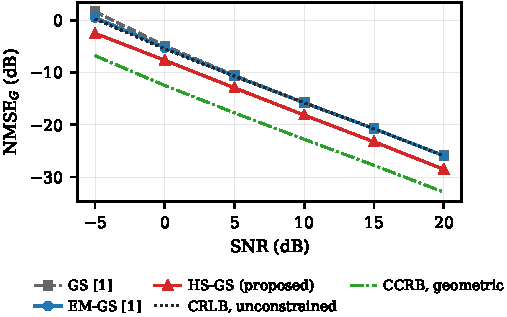
\includegraphics[width=0.93\columnwidth]{fig/fig1_nmse_vs_snr.pdf}\\[3pt]
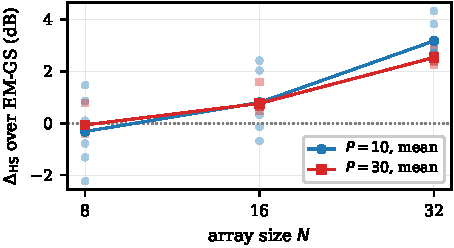
\includegraphics[width=0.93\columnwidth]{fig/fig2_gain_vs_N.pdf}
% SRC (both panels): results/track_b/b3/*.npz via scripts/plot_paper.py.
% Gain per N = mean over 12 operating points (2 pilot counts x 6 SNR).
\caption{\textbf{The gain is real but conditional.} [Family B3.]
\emph{Top:} NMSE versus SNR at $N=32$, $K=3$, $P=30$, RSR $=12$~dB, $400$
paired trials per point; HS-GS gains $2.27$--$3.04$~dB over EM-GS, and both
bounds are plotted for reference (neither governs a biased estimator).
\emph{Bottom:} mean gain over the $12$ operating points ($2$ pilot counts
$\times\,6$ SNR values) at each array size: $-0.19$, $+0.78$, $+2.85$~dB at
$N=8,16,32$. \textbf{The sign changes with aperture.}}
\label{fig:main}
\end{figure}

\subsection{Aperture: the gain is not universal}

Repeating the comparison across array sizes gives a mean gain over the $12$
operating points of
% SRC: results/track_b/b3/*.npz, mean over P in {10,30} x 6 SNR values.
$-0.19$, $+0.78$ and $+2.85$~dB at $N=8$, $16$ and $32$ [B3]
(Fig.~\ref{fig:main}, right). \textbf{The gain changes sign.}

At $N=8$ the capacity is $\rmax=4$ by \eqref{eq:cap} while the simulated path
counts satisfy $L_k\in\{3,\dots,7\}$, so the prior is frequently vacuous or
actively harmful: the projection is inactive in $42.5\%$ of trials [B3], and
where it is active it often truncates genuine components. The $N=8$ behaviour
is discussed further in Section~\ref{sec:limits}.

This raises the question that organises the rest of the work. Is array size
itself the operative variable, or is $N$ a proxy for something else? Capacity
\eqref{eq:cap} suggests the latter: what should matter is not $N$ alone but how
much of the available rank capacity the channel actually consumes.

\subsection{A controlled path-count experiment}

To separate the two, we fix $N=32$ and vary only the path count, with $L$ held
identical across users and everything else unchanged
(Fig.~\ref{fig:pathcount}). The gain decays monotonically from
% SRC: trackB_hankel_emgs/results/experiment_C_path_count.csv, gain_db column.
$+7.04$~dB at $L=2$ to $-0.12$~dB at $L=16=\rmax$ [EXT], reaching a null at
$L=14$ and turning significantly negative at $L=16$. Over the same sweep EM-GS
moves by $0.191$~dB in total [EXT] --- an estimator that ignores structure
should not respond to a change in structure, and it does not, which is the
control this experiment needs.

So the operative variable is channel complexity relative to capacity, not
aperture. Aperture matters only because it sets the capacity.

\subsection{Effective rank as the coordinate}

Raw path count is still an imperfect description of complexity. Two channels
with the same $L$ can occupy very different numbers of effective dimensions if
their paths are clustered in angle or unequal in strength, since near-collinear
or weak components contribute little to the Hankel spectrum. We therefore
replace $L$ by the effective rank of Roy and Vetterli \cite{royvetterli2007},
\begin{equation}\label{eq:reff}
\reff=\exp\Bigl(-\sum_i p_i\ln p_i\Bigr),\qquad
p_i=\sigma_i\Big/\textstyle\sum_j\sigma_j,
\end{equation}
computed on the Hankel lifting, and normalise it by capacity,
\begin{equation}\label{eq:rho}
\rho=\reff/\rmax(N)\in(0,1].
\end{equation}
$\rho$ measures the fraction of the available Hankel rank capacity the channel
actually occupies; $\rho\to1$ is the regime in which \eqref{eq:rank} says
nothing.

Plotted against $\rho$, gain curves measured at three different array sizes lie
close to one another and cross zero at
% SRC: reports/trackD_partB9_analysis.json, B1_collapse.zero_crossing_r_eff_over_cap
$\rho=0.588$, $0.518$ and $0.544$ for $N=16$, $32$ and $64$ [TD]
(Fig.~\ref{fig:boundary}) --- a spread of $0.070$ in $\rho$.

\textbf{This is an approximate scaling, not a collapse.} The \emph{location} of
the useful/not-useful boundary is stable across aperture; the gain
\emph{magnitude} is not. Comparing $N=16$ against $N=64$ over their region of
overlap in $\rho$ leaves a residual of mean $0.493$~dB and maximum $0.901$~dB
[TD], and that residual is one-signed rather than scattered, so it is a
systematic aperture dependence and not sampling noise. We report $\rho$ as the
coordinate that predicts \emph{whether} the prior helps, not one that predicts
\emph{how much} it helps to within the measurement error. Two of the three
crossings are also extrapolated rather than bracketed by a measured sign change
($N=32$ is bracketed; $N=16$ and $N=64$ are not).

\begin{figure}[!t]
\centering
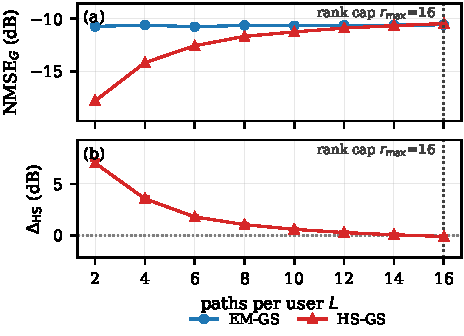
\includegraphics[width=0.90\columnwidth]{fig/fig3_pathcount.pdf}
% SRC: trackB_hankel_emgs/results/experiment_C_path_count.csv
\caption{\textbf{Path count is the operative variable, not aperture.}
[Family EXT.] Controlled sweep at $N=32$, $K=3$, $P=30$, SNR $=5$~dB, $300$
trials per point, $L$ fixed and identical across users. (a) EM-GS is flat in
$L$ ($0.191$~dB total) while HS-GS rises to meet it. (b) The paired gain decays
from $+7.04$~dB at $L=2$ to $-0.12$~dB at $L=16=\rmax$; the $95\%$ bootstrap
band is narrower than the markers. The hypothesis was recorded before the run.}
\label{fig:pathcount}
\end{figure}

\begin{figure}[!t]
\centering
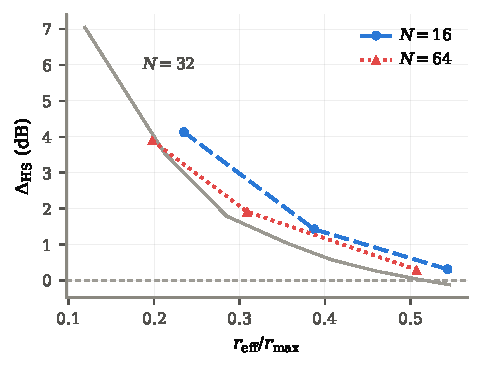
\includegraphics[width=0.90\columnwidth]{fig/fig7_boundary_invariance.pdf}
% SRC: reports/trackD_partB9_analysis.json, B1_collapse.delta_by_N
\caption{\textbf{Effective rank is the coordinate.} [Family TD.] The same gain
plotted against $\rho=\reff/\rmax$ for $N\in\{16,32,64\}$, crossing zero at
$\rho=0.588/0.518/0.544$. The boundary \emph{location} is what is stable
across aperture; a one-signed magnitude residual remains (\S\ref{sec:limits}).}
\label{fig:boundary}
\end{figure}

\subsection{Prospective cross-generator validation}

A relation fitted and then evaluated on the same data proves little. We
therefore froze the $\rho$-to-gain relation obtained from the ULA experiments
above, committed numerical predictions to version control, and only then ran
two channel generators that had played no part in constructing it. The
relation was \emph{not} refitted afterwards. The prediction rule is a
piecewise-linear interpolation on a fixed eight-point table --- no regression
and no spline --- so it can be re-executed exactly.

\emph{Generator 1: clustered Saleh--Valenzuela.} The clustered multipath model
associated with the configuration of Xiao \emph{et al.} \cite{xiao2026}, which
follows the description in \cite{meijerink2014}. At $\rho=0.331$ the frozen
relation predicted $\dHS=+1.30$~dB; the measurement over $276$ trials gave
% SRC: reports/trackD_partB9_analysis.json, B6_xiao.B6_xiao_clustered
$+1.173$~dB with $95\%$ CI $[+1.017,+1.380]$ --- an error of $0.13$~dB [TD].

\emph{Generator 2: the $L=10$ configuration.} The simulation configuration
reported in \cite{precoding2408}. At $\rho=0.400$ the prediction was
$+0.648$~dB with a stated interval $[+0.367,+1.015]$; the measurement over
$266$ trials gave
% SRC: reports/trackD_partB9_analysis.json, B8_cui_measured
$+0.963$~dB with $95\%$ CI $[+0.808,+1.086]$ --- an error of $0.315$~dB, inside
the stated prediction interval but on its upper edge [TD].

\textbf{What this does and does not show.} These are \emph{cross-generator} or
distribution-shift tests, not out-of-model tests: both generators still produce
channels of the form \eqref{eq:chan}, and only the distribution over
$(L_k,\alpha_{\ell,k},\theta_{\ell,k})$ changes. So this is evidence that
$\rho$ transfers across path distributions, not that it survives a violation of
the ULA sum-of-exponentials model. Within that scope, a frozen coordinate
predicted a structural gain on unseen channel statistics to $0.13$ and
$0.315$~dB, and the weaker second case is reported alongside the first.

\begin{figure}[!t]
\centering
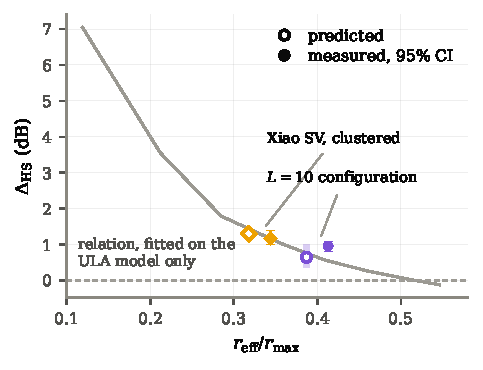
\includegraphics[width=0.86\columnwidth]{fig/fig8_cross_generator.pdf}
% SRC: reports/trackD_step0_cui_prediction.json (committed before measurement)
% and reports/trackD_partB9_analysis.json (measurements).
\caption{\textbf{Predictions registered before measurement.} [Family TD,
$N=32$, $K=3$, $P=20$, adaptive order, $n_{\mathrm{cz}}=1$,
SNR $\sim\mathcal{U}[-10,20]$~dB.] Hollow markers are what the frozen relation
predicted; filled markers with bars are what was measured, with $95\%$
confidence intervals. The grey curve is the relation itself, fitted on the ULA
experiments only and not refitted for either generator. The two are drawn at a
small horizontal offset because at the same abscissa they overlap --- which is
the result, but would hide which is which. Errors: $0.13$~dB (clustered
Saleh--Valenzuela, $276$ trials) and $0.315$~dB ($L=10$ config., $266$ trials).}
\label{fig:pred}
\end{figure}

% =====================================================================
\section{Limitations}\label{sec:limits}
% =====================================================================

These define the regime in which the method is useful and are reported in full.

\textbf{$N=8$ is a mixed result, not a small positive one.} The gain is
% SRC: results/track_b/b3/N8_P{10,30}_snr*.npz
$+1.47$~dB at $-5$~dB SNR ($P=10$) but falls to $-2.23$~dB at high SNR [B3],
because truncation bias does not shrink with noise: as SNR rises the variance
term falls while the bias term does not, so the trade stops paying and then
reverses. The sign of any single scalar summary at $N=8$ depends on the pooling
rule, which is why per-point values are reported.
\textbf{The effective-rank scaling is approximate.} The boundary location is
stable across aperture; the gain magnitude is not, leaving an unexplained
one-signed residual of mean $0.493$~dB (maximum $0.901$~dB) between $N=16$ and
$N=64$ [TD]. \textbf{A pre-registered criterion narrowly failed.} A
% SRC: reports/trackD_partB9_analysis.json, cells B2_K{2,3,4}
$K$-invariance test at fixed pilot adequacy $P/2K=3.33$ passes comfortably at
SNR $\ge5$~dB (spread $0.094$~dB) but, pooled over all SNR, gives $0.294$~dB
against a falsifier registered at $0.3$~dB --- missed by $0.006$~dB [TD];
reported rather than dropped. \textbf{Simulation only.} No measured hardware
and no recorded channel data; the atomic response enters only through
\eqref{eq:obs}, and all channels are geometric ULA channels of the form
\eqref{eq:chan}. \textbf{Order selection is expensive}, accounting for
% SRC: results/track_b/timing.json, order_search_share
$57.7$--$85.5\%$ of HS-GS runtime [B3]; a coarse-to-fine search or reuse of
$\hat L$ across coherence blocks is the obvious target, and neither was
attempted. \textbf{Neither bound governs the estimators compared to them}, as
noted in \S\ref{sec:results}-A.

% =====================================================================
\section{Conclusion}
% =====================================================================

Hankel structural regularisation can substantially improve magnitude-only
Rydberg channel estimation, but only when the channel occupies a sufficiently
small fraction of the array's Hankel rank capacity: we observe
$+2.27$ to $+3.04$~dB at $N=32$, $P=30$ [B3], and a sign reversal at $N=8$.
The more general finding is that the normalised effective rank
$\rho=\reff/\rmax$ is more informative than raw path count or array size alone
in describing when the structural prior is useful --- a controlled sweep at
fixed $N$ drives the gain from $+7.04$ to $-0.12$~dB as $L$ approaches capacity
[EXT], and the zero crossing in $\rho$ sits within a spread of $0.070$ across
three array sizes [TD]. Two frozen cross-generator predictions were met to
$0.13$ and $0.315$~dB, which is preliminary predictive evidence rather than a
validated scaling law: the magnitude residual across aperture is unexplained,
one pre-registered criterion narrowly failed, and every result here is
simulation-only on geometric ULA channels. Broader channel families,
non-idealities of a physical vapour cell, and measurements on hardware are all
required before the coordinate can be claimed to generalise.

\begin{thebibliography}{99}
\bibitem{gong2025mag} T.~Gong \emph{et al.}, ``Rydberg atomic quantum receivers
for classical wireless communication and sensing,'' \emph{IEEE Wireless
Commun.}, vol.~32, no.~5, pp.~90--100, 2025.

\bibitem{gerchberg1972} R.~W.~Gerchberg and W.~O.~Saxton, ``A practical
algorithm for the determination of phase from image and diffraction plane
pictures,'' \emph{Optik}, vol.~35, pp.~237--246, 1972.

\bibitem{cui2025} M.~Cui, Q.~Zeng, and K.~Huang, ``Towards atomic MIMO
receivers,'' \emph{IEEE J. Sel. Areas Commun.}, vol.~43, no.~3, pp.~659--673,
2025.

\bibitem{xu2025} B.~Xu, J.~Zhang, Z.~Chen, B.~Cheng, Z.~Liu, Y.-C.~Wu, and
B.~Ai, ``Channel estimation for Rydberg atomic receivers,'' \emph{IEEE Wireless
Commun. Lett.}, vol.~14, no.~9, pp.~2957--2961, 2025.

\bibitem{cadzow1988} J.~A.~Cadzow, ``Signal enhancement---a composite property
mapping algorithm,'' \emph{IEEE Trans. Acoust., Speech, Signal Process.},
vol.~36, no.~1, pp.~49--62, 1988.

\bibitem{markovsky2008} I.~Markovsky, ``Structured low-rank approximation and
its applications,'' \emph{Automatica}, vol.~44, no.~4, pp.~891--909, 2008.

\bibitem{royvetterli2007} O.~Roy and M.~Vetterli, ``The effective rank: a
measure of effective dimensionality,'' in \emph{Proc. Eur. Signal Process.
Conf. (EUSIPCO)}, 2007, pp.~606--610.

\bibitem{gorman1990} J.~D.~Gorman and A.~O.~Hero, ``Lower bounds for parametric
estimation with constraints,'' \emph{IEEE Trans. Inf. Theory}, vol.~36, no.~6,
pp.~1285--1301, 1990.

\bibitem{stoica1998} P.~Stoica and B.~C.~Ng, ``On the Cram\'er--Rao bound under
parametric constraints,'' \emph{IEEE Signal Process. Lett.}, vol.~5, no.~7,
pp.~177--179, 1998.

\bibitem{xiao2026} J.~Xiao, J.~Wang, M.~Zeng, H.~Xu, X.~Li, and
A.~Nallanathan, ``Channel estimation for Rydberg atomic quantum receivers:
unrolled phase retrieval from holographic snapshots,'' \emph{IEEE Signal
Process. Lett.}, vol.~33, pp.~1696--1700, 2026.

\bibitem{meijerink2014} A.~Meijerink and A.~F.~Molisch, ``On the physical
interpretation of the Saleh--Valenzuela model and the definition of its power
delay profiles,'' \emph{IEEE Trans. Antennas Propag.}, vol.~62, no.~9,
pp.~4780--4793, 2014.

\bibitem{precoding2408} M.~Cui, Q.~Zeng, and K.~Huang, ``MIMO precoding for
Rydberg atomic receivers,'' 2024, arXiv:2408.14366.
\end{thebibliography}

\end{document}
